%%
%% Author: Alicia Zamorano
%% 21-04-18
%%

% Preamble
\documentclass[11pt]{article}

% Packages
\usepackage{graphicx}
\usepackage{float}
\graphicspath{ {../images/} }

% Document
\begin{document}
\title{Concurrency between Entity Relationship and Object Oriented Paradigm}
\author{Alicia Zamorano}
\maketitle
\section{Introduction}

The relational model has it's bases on a mathematical concept know as relation and it
describes a precise set of data manipulation constructs based on advanced mathematical
concepts.\cite{data_base_sys}
The relational data model is a result of the work that Edgar Codd made during the 1960s\cite{relational_db_design_and_impl}.
In mathemathical set theory a relation is the definition of a table with columns(attributes) and rows(tuples) and this relations have specific
characterisics which are described following:\\
\textbf{Columns} a column has the following properties
\begin{itemize}
	\item Unique name
	\item Domain. Each column has a domain, an expression of  the permissible values for that attribute.
	      almost all the DBMS enforces a domian through a \textit{domain constraint}. A domain is defined over types
	      where a type is a set of values, for instance the type INTEGER
	      for the set of all the integers, or the CHAR for the set of all the character strings.
	\item Any order
\end{itemize}\\
\textbf{Rows} a row in a relation has the following properties
\begin{itemize}
	\item Univaluated attributes.
	\item Uniqueness, there should not be duplicated rows in a relation
	\item Primary Key, is a column or combination of columns with a value that identifies uniquely each row.
	\item No positional concept.
\end{itemize}
To be able to retrieve any single piece of data from a data base three things are necessary, the name of the table, the name
of the column and the primary key of the row.\\ In relational data bases is not permitted to set a value of a primary key as \textit{null}
or blank, this constraint is known as \textit{entity integrity} the primary keys should have three desirable properties:

\begin{enumerate}
	\item A primary key should have a value that is highly unlikely to be ever null.
	\item A primary key value should never change.
	\item A primary key should avoid using meaninful data.
\end{enumerate}

\textit{Entity-relationship} (ER) \textit{diagrams} (ERDs) provides a way to document the entities in a database along with the types
defined in that entities. There are three mayor methods to represent ER diagrams:

\begin{enumerate}
	\item \textbf{Chen Model} (named in honor of the originator of ER modeling Dr.P.S Chen)\\
	      Represents the entities with squares and uses diamonds for relationships, and lines with arrows
	      to indicate the relationships between the entities.

	      \begin{figure}[H]
	      	\centering
	      	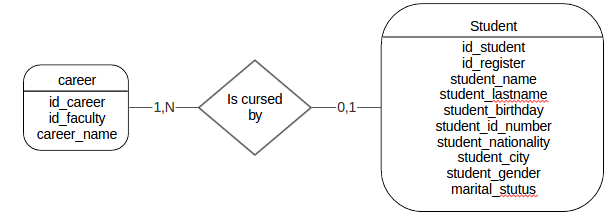
\includegraphics[width=12cm]{peterchennotation}
	      	\caption{A Chen ER diagram showing relationship between an Student and his/her careers.}
	      \end{figure}

	\item \textbf{Information Engineering} (IE. or "crows feet")\\
	      Uses squares to represent the entities and uses lines to represent the relationship, however in this
	      case the ends of the lines(the ones that looks like a bird foot are often called "crows feet" ) indicates which relationships are mandatory\\
	      There are four symbols used at the end of the lines:\\

	      \textbf{\textbar\textbar:} One and one only (Mandatory relationship)\\
	      \textbf{0 \textbar:} Zero or one\\
	      \textbf{\textgreater 1:} One or more (Mandatory relationship)\\
	      \textbf{\textgreater 0:} Zero, one, or more\\

	      \begin{figure}[H]
	      	\centering
	      	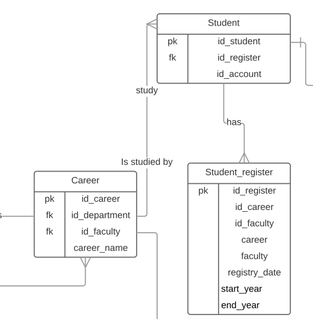
\includegraphics[width=8cm]{crowsfeet}
	      	\caption{Example of ERD diagram using Crow's Feet Model.}
	      \end{figure}

	\item \textbf{Unified Modeling Languague (UML)} very similar to IE notation.The symbols at the end of the lines
	      are replaced by numeric representations of the type of relationship. There are four possible relationships:\\

	      \textbf{1: } One and only one (mandatory) \\
	      \textbf{1...*} One or more (mandatory)    \\
	      \textbf{0...1} Zero or one                \\
	      \textbf{0...*} Zero, one, or more         \\

	      \begin{figure}[H]
	      	\centering
	      	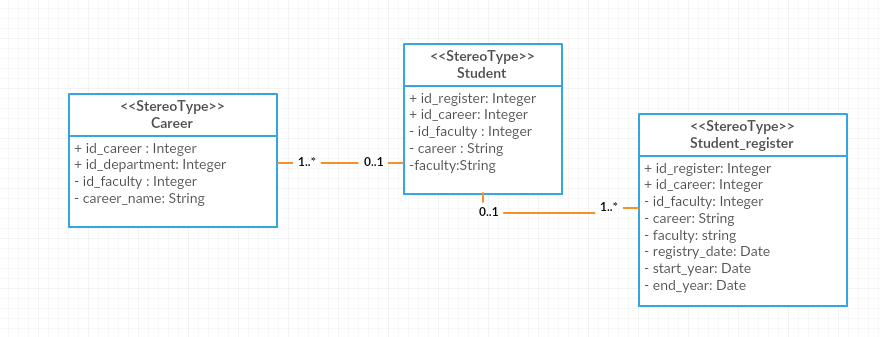
\includegraphics[width=8cm]{UML}
	      	\caption{Example of ERD diagram using UML.}
	      \end{figure}
\end{enumerate}

In the other hand Object Oriented(Futhermore cited as OO) Systems are typically characterized by four basic components: Identity, state, behavior
and encapsultaion.\\

\textbf{Identity} A given object has a unique identifier that is implicitly defined, in most OO languages that is distinct from its state.\\
\textbf{State} An object has a defined state, the attributes defined at the moment of the creation of an object. Two objects can have the same state
and still be different from each other. There is a well known disscussion "indentity vs equivalence".\\
\textbf{Behavior} It is possible to define, invoke, manipulate and interact with operations over objects.\\
\textbf{Encapsulation} Is a key feature of objects that prevents the manipulation of internal details of an object from outside clients that has access
to object interfaces.\\

To work with Entity Relationship models and object oriented paradigm a technique called ORM(Object Relational Mapping) had been created
this technique allows to map the objects to entities and the Entities to Objects and viceversa.
\medskip
\begin{thebibliography}{9}
	\bibitem{data_base_sys}
	Peter Rob, Carlos Coronel(2009).
	\textit{Database systems design, implementation, and management. Boston, Massachusetts:Thomson ISBN-13: 978-1-4239-0201-0.}
	\bibitem{relational_db_design_and_impl}
	Jan L. Harrington(2009).
	\textit{Relational Database Design and Implementation. Burlington USA:Morgan Kaufmann. ISBN:978-0-12-374730-3.}
\end{thebibliography}
\end{document}
